\documentclass[aspectratio=169,9pt]{beamer}

\usepackage[utf8]{inputenc}
\usepackage{graphicx}
\graphicspath{ {./figures/} }
\usepackage{caption}
\captionsetup{font=tiny,labelfont=tiny}
\usepackage[maxbibnames=9,maxcitenames=1,doi=false,isbn=false,url=false,eprint=false,citestyle=authoryear]{biblatex}
\usepackage{hyperref}

% Beamer dark theme
\setbeamercolor{normal text}{fg=white,bg=black!90}
\setbeamercolor{structure}{fg=white}
\setbeamercolor{alerted text}{fg=red!85!black}
\setbeamercolor{item projected}{use=item,fg=black,bg=item.fg!35}
\setbeamercolor*{palette primary}{use=structure,fg=structure.fg}
\setbeamercolor*{palette secondary}{use=structure,fg=structure.fg!95!black}
\setbeamercolor*{palette tertiary}{use=structure,fg=structure.fg!90!black}
\setbeamercolor*{palette quaternary}{use=structure,fg=structure.fg!95!black,bg=black!80}
\setbeamercolor*{framesubtitle}{fg=white}
\setbeamercolor*{block title}{parent=structure,bg=black!60}
\setbeamercolor*{block body}{fg=black,bg=black!10}
\setbeamercolor*{block title alerted}{parent=alerted text,bg=black!15}
\setbeamercolor*{block title example}{parent=example text,bg=black!15}

\addtobeamertemplate{navigation symbols}{}{%
    \usebeamerfont{footline}%
    \usebeamercolor[fg]{footline}%
    \hspace{1em}%
    \insertframenumber/\inserttotalframenumber
}


%Information to be included in the title page:
\title{Studying the effects of competition on adaptive therapy}
\subtitle{Mid Year Presentation}
\author{Harshavardhan BV (20161100)\\ 5th Year BS-MS}
\date{January 2021}
\institute{Under the guidance of Prof. Sutirth Dey,\\ IISER Pune}

\bibliography{References}

\begin{document}

\frame{\titlepage}

\section{Introduction}
\begin{frame}{Adaptive Therapy}
  \begin{itemize}
    \item Conventional therapy @ MTD $\rightarrow$ min tumour burden
    \item Heterogenous sensitivity $\rightarrow$ sensitive eliminated $\rightarrow$ resistant population (\cite{Scott})
    \item AT = lower, fluctuating dose $\rightarrow$ sensitive preserved
  \end{itemize}
\end{frame}

\begin{frame}{mCRPC}
  \begin{itemize}
    \item System of study: Metastatic Castration-Resistant Prostate Cancer
    \item History of Adaptive therapy work (\cite{Cunningham})
    \item Therapy: ADT + abiraterone
  \end{itemize}
  \begin{table}
    \centering
    \begin{tabular}{|l|c|c|c|}
    \hline
    Cell type & Test. dependent & Test. Producing & Mechanism \\
    \hline
    $T^+$ & Yes & No & N/A \\
    $T^p$ & Yes & Yes & Cholestrol $\xrightarrow{CYP17\alpha}$ Testosterone\\
    $T^-$ & No & No & Androgen receptor mutations\\
    \hline
    \end{tabular}
  \end{table}
\end{frame}

\begin{frame}{Competition between cells}
  \begin{itemize}
    \item AT outcome $\sim$ competition b/w sensitive and resistant
    \item Competitive strategies through traits from cancer progression (\cite{Hanahan})
    \begin{itemize}
      \item Higher proliferation rate
      \item Better survival @ sub-optimal conditions
      \item Lower death rate
    \end{itemize}
  \end{itemize}
\end{frame}

\section{Work Done}
\begin{frame}{ODE Model}
  \begin{columns}
    \begin{column}{0.4\textwidth}
      \begin{itemize}
        \item Starting point: forming expectations, parameterization for ABM
        \item Computationally cheap but can't capture complex behaviour
        \item Logistic framework with dynamic carrying capacity $\sim$ environmental conditions
        \item Environment = resource = \{oxygen, testosterone\}
      \end{itemize}
    \end{column}
    \begin{column}{0.6\textwidth}
      \begin{equation}
        \frac{dy_i}{dt} = r_i y_i (1 - \frac{\sum_j y_j}{1 + K_{i,max} f_i(O_2) f_i(test)} )- \delta_i y_i
        \label{celleq}
      \end{equation}
      \begin{equation}
        \frac{dO_2}{dt} = p_{O_2} - \sum_i \mu_{O_2,i} y_i - \lambda_{O_2} O_2
        \label{o2eq}
      \end{equation}
      \begin{equation}
        \frac{dtest}{dt} = p_{test} y_{T^p} - \sum_i \mu_{test,i} y_i - \lambda_{test} test
        \label{testeq}
      \end{equation}
      \begin{equation}
        f_i(res) = \begin{cases}
          1 &\text{if } ul_{res,i} \leq res\\
          \frac{res-ll_{res,i}}{ul_{res,i}-ll_{res,i}} &\text{if } ll_{res,i} < res < ul_{res,i}\\
          0 &\text{if } res \leq ll_{res,i}\\
        \end{cases}
        \label{freseq}
      \end{equation}
      $i \in \{T^+,T^p,T^-\}$ and $res \in \{O_2,test\}$.
    \end{column}
  \end{columns}
\end{frame}

\begin{frame}{Parameters \& Standardization}
  Some parameters directly from literature
  \begin{itemize}
    \item $\delta_i$: Death rate (\cite{Jain})\\
    \begin{tabular}{ll}
      $T^+$ & $2.5 \times 10^{-3}$ min$^{-1}$\\
      $T^p$ & $2.5 \times 10^{-3}$ min$^{-1}$\\
      $T^-$ & $1.6 \times 10^{-4}$ min$^{-1}$\\
    \end{tabular}
    \item $\mu_{O_2,i}$: Oxygen uptake (\cite{HailJr})\\
    \begin{tabular}{ll}
      $T^+$ & $1.63 \times 10^{-6}$ min$^{-1}$cell$^{-1}$\\
      $T^p$ & $1.63 \times 10^{-6}$ min$^{-1}$cell$^{-1}$\\
      $T^-$ & $1.04 \times 10^{-6}$ min$^{-1}$cell$^{-1}$\\
    \end{tabular}
    \item $\lambda_{res}$: Decay rate (\cite{Jain})\\
    \begin{tabular}{ll}
      $O_2$ & 0.100 min$^{-1}$\\
      $test$ & 0.004 min$^{-1}$\\
    \end{tabular}
  \end{itemize}
\end{frame}
\begin{frame}{Parameters \& Standardization}
  Some additional supplementary parameters
  \begin{itemize}
    \item $\tau_d$: Doubling time (\cite{atcc})\\
    \begin{tabular}{ll}
      $T^+$ & $34$ hr \\
      $T^p$ & $40$ hr \\
      $T^-$ & $25$ hr \\
    \end{tabular}
    \item $y_i^*$: Equilibrium cell number (assumed)\\
    10000
    \item $res^*$: Equilibrium/Tissue resource levels (\cite{Steward},\cite{Titus})\\
    \begin{tabular}{ll}
      $O_2$    & 2.5 mmHg          \\
      $test$   & 3.74 pmol/g tissue\\
    \end{tabular}
  \end{itemize}
\end{frame}
\begin{frame}{Parameters \& Standardization}
  Some parameters from assumptions \& constraints
  \begin{columns}
    \begin{column}{0.5\textwidth}
      \begin{itemize}
        \item $r_i$: Growth rate (Eq \ref{r_eq})\\
        \begin{tabular}{ll}
          $T^+$ & $2.84 \times 10^{-3}$ min$^{-1}$\\
          $T^p$ & $2.79 \times 10^{-3}$ min$^{-1}$\\
          $T^-$ & $6.23 \times 10^{-4}$ min$^{-1}$\\
        \end{tabular}
        \item $K_{i,max}$: Maximum Carrying capacity (Eq \ref{rho_eq})\\
        \begin{tabular}{ll}
          $T^+$ & $8.35 \times 10^4$ \\
          $T^p$ & $9.62 \times 10^4$ \\
          $T^-$ & $1.34 \times 10^4$ \\
        \end{tabular}
        \item $p_{res}$: Production rate (Eq \ref{p_o2_eq},\ref{p_test_eq})\\
        \begin{tabular}{ll}
          $O_2$ & 0.11 min$^{-1}$\\
          $test$ & $5 \times 10^{-7}$ min$^{-1}$cell$^{-1}$\\
        \end{tabular}
        \item $\mu_{test,i}$: Testosterone uptake (Eq \ref{p_test_eq})\\
        \begin{tabular}{ll}
          $T^+$ & $2.34 \times 10^{-8}$ min$^{-1}$cell$^{-1}$\\
          $T^p$ & $6.00 \times 10^{-8}$ min$^{-1}$cell$^{-1}$\\
          $T^-$ & 0 min$^{-1}$cell$^{-1}$\\
        \end{tabular}
        \item $ll_{res,i}$: Lower limit/threshold level
        $\in [0,1]$
        \item $ul_{res,i}$: Upper limit/saturation level
        $\in [0,1]$
      \end{itemize}
    \end{column}
    \begin{column}{0.5\textwidth}
      \begin{equation}
        r_i = \frac{ln(2)}{\tau_{d,i}} + \delta_i
        \label{r_eq}
      \end{equation}
      \begin{equation}
        K_{i,max}=\frac{r_i}{r_i-\delta_i} y_i^*
        \label{rho_eq}
      \end{equation}
      \begin{equation}
        p_{O_2} = \lambda_{O_2} O_2^* + y_i^* \mu_i
        \label{p_o2_eq}
      \end{equation}
      \begin{equation}
        p_{test} - \mu_{test,T^p} = \frac{test^* \lambda_{test}}{y_{T^p}^*} = 4 \times 10^{-4}
        \label{p_test_eq}
      \end{equation}
    \end{column}
  \end{columns}
\end{frame}

\subsubsection{Pairwise Competition}
\begin{frame}{Pairwise Competition: $T^p - T^-$}
  \begin{columns}
    \begin{column}{0.5\textwidth}
      \begin{enumerate}
        \item<1-> $T^p$ $test$ \& $O_2$ limited. $T^-$ only $O_2$ limited
          \begin{itemize}
            \item Testosterone limitation $\sim$ $ll_{test,T^p}$ and $ul_{test,T^p}$
          \end{itemize}
        \item<2-> $ul_{test,T^p}$ low
        \begin{itemize}
          \item $T^p$ not severely testosterone limited
          \item $T^p$ coexist or outcompete $T^-$
          \item $T^-$ Outcompetes in other cases
        \end{itemize}
        \item<3-> $ll_{O_2,T^-}$ large
        \begin{itemize}
          \item $T^-$ strongly oxygen limited
          \item $T^p$ still testosterone limited
          \item $T^-$ wins eventually
          \item Oxygen levels rise faster than testosterone
        \end{itemize}
        \item<4-> Outcomes dependent on the initial proportion of $T^p$
      \end{enumerate}
    \end{column}
    \begin{column}{0.5\textwidth}
      \begin{figure}[h]
        \centering
        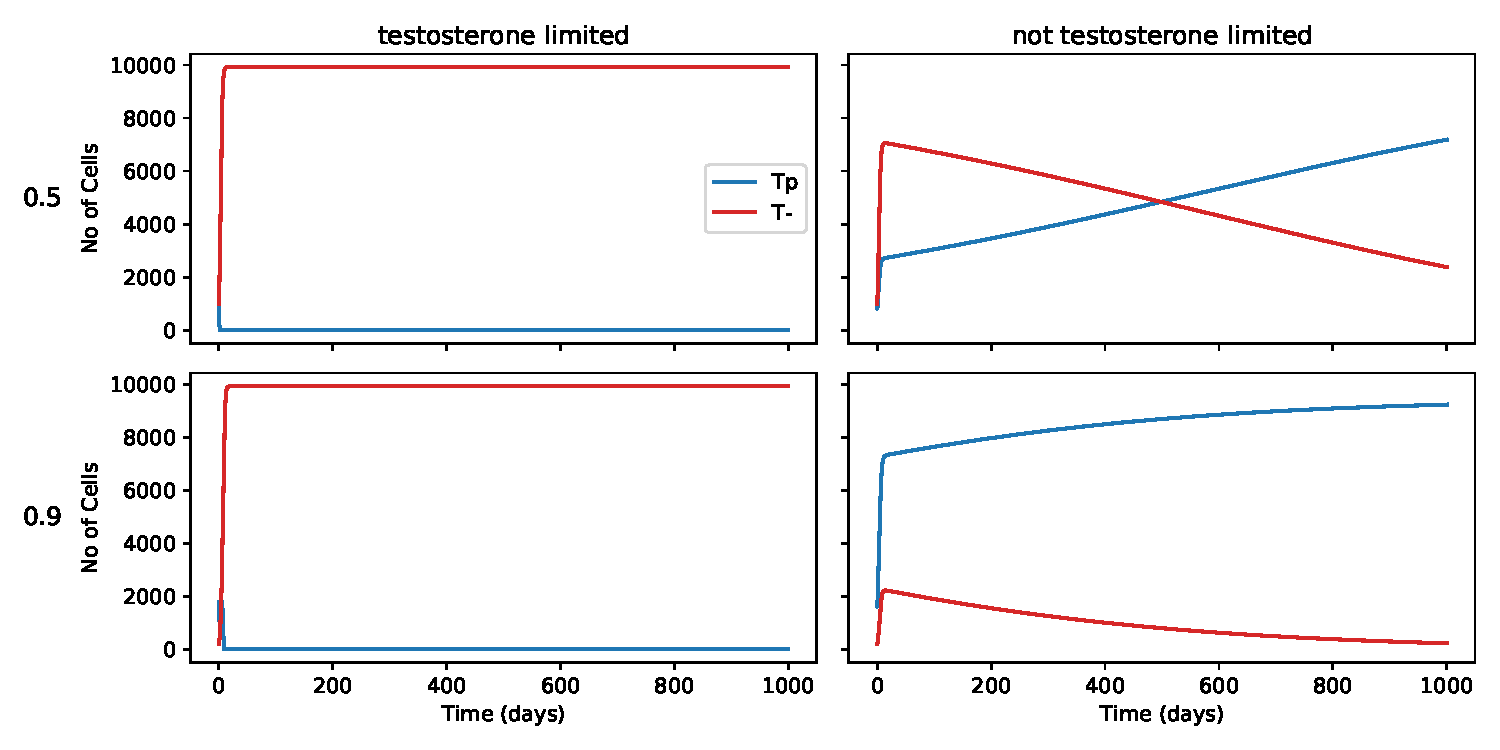
\includegraphics[width=\textwidth]{Tpro-Tneg}
        \caption{Pairwise $T^p - T^-$ timeseries, when $T^p$ is testosterone limited and not testosterone limited (colums) and at different initial proportions of $T^p$(rows)}
        \label{fig_Tpro-Tneg}
      \end{figure}
    \end{column}
  \end{columns}
\end{frame}

\begin{frame}{Pairwise Competition: $T^+ - T^p$}
  \begin{columns}
    \begin{column}{0.6\textwidth}
      \begin{enumerate}
        \item<1-> Both cell type limited by both resource
        \& strength of limitation of resource through limits
        \item<2-> Both severly testosterone limited
        \begin{itemize}
          \item $T^+$ consume \& grows on limited testosterone
          \item Density-dependent competition drive $T^p$ extinct
          \item No $T^p$ = No testosterone $\rightarrow$ $T^+$ extinct
        \end{itemize}
        \item<3-> $ll_{O_2,T^p}$ large
        \begin{itemize}
          \item $T^+$ severly oxygen limited
          \item $T^p$ grow initially \& secrete testosterone
          \item Sustain small $T^+$ if not extinct
        \end{itemize}
        \item<4-> $ul_{test,T^p} \leq ul_{test,T^+}$
        \begin{itemize}
          \item $T^p$ is weakly limited by testosterone relative to $T^+$
          \item Both coexist
          \item $T^p$ grow initially \& not affected by $T^+$
        \end{itemize}
      \end{enumerate}
    \end{column}
    \begin{column}{0.4\textwidth}
      \begin{figure}[h]
        \centering
        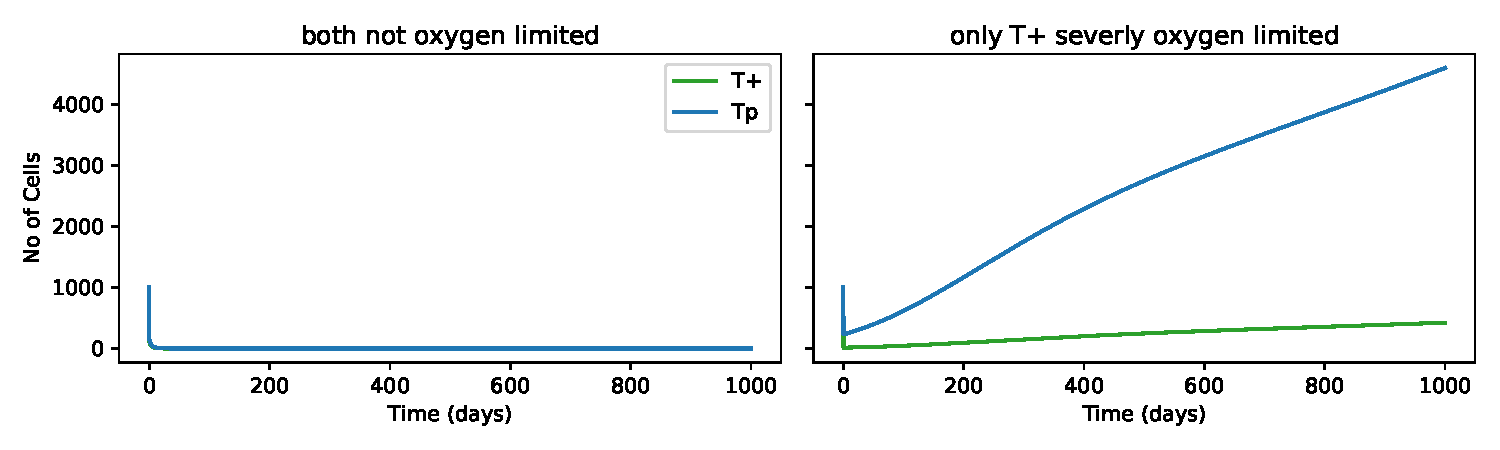
\includegraphics[width=\textwidth]{Tpos-Tpro_o2lims}
        \caption{Pairwise $T^+ - T^p$ timeseries, when both cell types are testosterone limited and not oxygen limited and when $T^+$ is severly oxygen limited}
        \label{fig_Tpos-Tpro_o2lims}
      \end{figure}
      \begin{figure}[h]
        \centering
        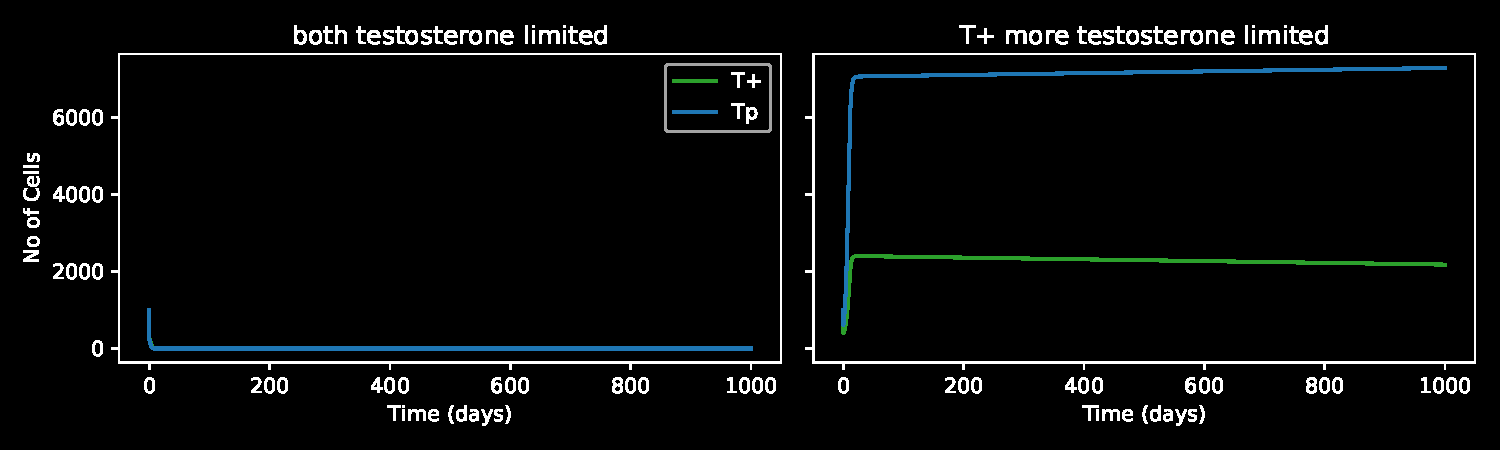
\includegraphics[width=\textwidth]{Tpos-Tpro_testlims}
        \caption{Pairwise $T^+ - T^p$ timeseries, when both cell types are testosterone limited and when $T^+$ is limited more than $T^p$}
        \label{fig_Tpos-Tpro_testlims}
      \end{figure}
    \end{column}
  \end{columns}
\end{frame}

\section{Future Plans}
\begin{frame}{Future Plans}
  \begin{itemize}
    \item Testosterone limitation relaxed
    \item Oxygen limit exploration with lower $ul_{test,i}$
    \item Make oxygen more limiting than testosterone via production rates
    \item 3 cell-type competition
    \item Simulate AT regimens with therapy as $p_{test} = f(dose)$
    \item Replicate in ABM \& Compare
  \end{itemize}
\end{frame}

\begin{frame}[allowframebreaks]{References}
  \printbibliography
\end{frame}

\end{document}
